There are several visualization tools that can be used for \amrex\
plotfiles.  The popular \visit\ package supports the \amrex\ file 
format natively (using the {\sf BoxLib2d} and {\sf BoxLib3d} file types),
as does the \yt\ python package.  The standard tool used within the
\amrex-community is \amrvis, a package developed and supported 
by CCSE that is designed specifically for highly efficient visualization
of block-structured hierarchical AMR data.

\section{\amrvis}

Our favorite visualization tool is \amrvis. We heartily encourage you
to build the {\tt amrvis2d} and {\tt amrvis3d} executables, and to try using them
to visualize your data. A very useful feature is View/Dataset, which
allows you to actually view the numbers in a spreadsheet that is nested
to reflect the AMR hierarchy -- this can be handy for
debugging. You can modify how many levels of data you want to see,
whether you want to see the grid boxes or not, what palette you use,
etc.  Here are some instructions and tips for using \amrvis:

\begin{enumerate}

\item Download and build \amrvis:
\begin{verbatim}
git clone https://ccse.lbl.gov/pub/Downloads/Amrvis.git
\end{verbatim}

Then {\tt cd} into {\tt Amrvis/}, edit the {\tt GNUmakefile} by
setting {\tt COMP} to the compiler suite you have.

Type {\tt make DIM=2} or {\tt make DIM=3} to build, 
resulting in an executable that looks like {\tt amrvis2d...ex}.

If you want to build amrvis with {\tt DIM=3}, you must first
download and build {\tt volpack}:
\begin{verbatim}
git clone https://ccse.lbl.gov/pub/Downloads/volpack.git
\end{verbatim}

Then {\tt cd} into {\tt volpack/} and type {\tt make}.

Note: \amrvis\ requires the OSF/Motif libraries and headers. If you don't have these 
you will need to install the development version of motif through your package manager. 
{\tt lesstif} gives some functionality and will allow you to build the amrvis executable, 
but \amrvis\ may exhibit subtle anomalies.

On most Linux distributions, the motif library is provided by the
{\tt openmotif} package, and its header files (like {\tt Xm.h}) are provided
by {\tt openmotif-devel}. If those packages are not installed, then use the
OS-specific package management tool to install them. 

You may then want to create an alias to {\tt amrvis2d}, for example
\begin{verbatim}
alias amrvis2d /tmp/Amrvis/amrvis2d...ex
\end{verbatim}

\item Run the command {\tt cp Amrvis/amrvis.defaults \textasciitilde/.amrvis.defaults}.
Then, in your copy, edit the line containing ``{\tt palette}'' line to point to, e.g., 
``{\tt palette  /home/username/Amrvis/Palette}''.  The other lines control
options such as the initial field to display, the number format, widow size, etc.
If there are multiple instances of the same option, the last option takes precedence.

\item Generally the plotfiles have the form {\tt pltXXXXX} 
  (the {\tt plt} prefix can be changed), where {\tt XXXXX} is a number 
  corresponding to the timestep the file
  was output.  {\tt amrvis2d <filename>} or {\tt amrvis3d <filename>}
  to see a single plotfile, 
  or for 2D data sets, {\tt amrvis2d -a plt*}, which will animate the 
  sequence of plotfiles.

  You can use the ``Variable'' menu to change the variable.
  You can left-click drag a box around a region
  and click "View'' $\rightarrow$ ``Dataset''
  in order to look at the actual numerical values
  (see Figure \ref{Fig:Amrvis}).
  Or you can simply left click on a point to obtain the numerical value.
  You can also export the
  pictures in several different formats under "File/Export".
  In 2D you can right and center click to get line-out plots.
  In 3D you can right and center click to change the planes, and the hold
  shift+(right or center) click to get line-out plots.

\begin{figure}[tb]
\centering
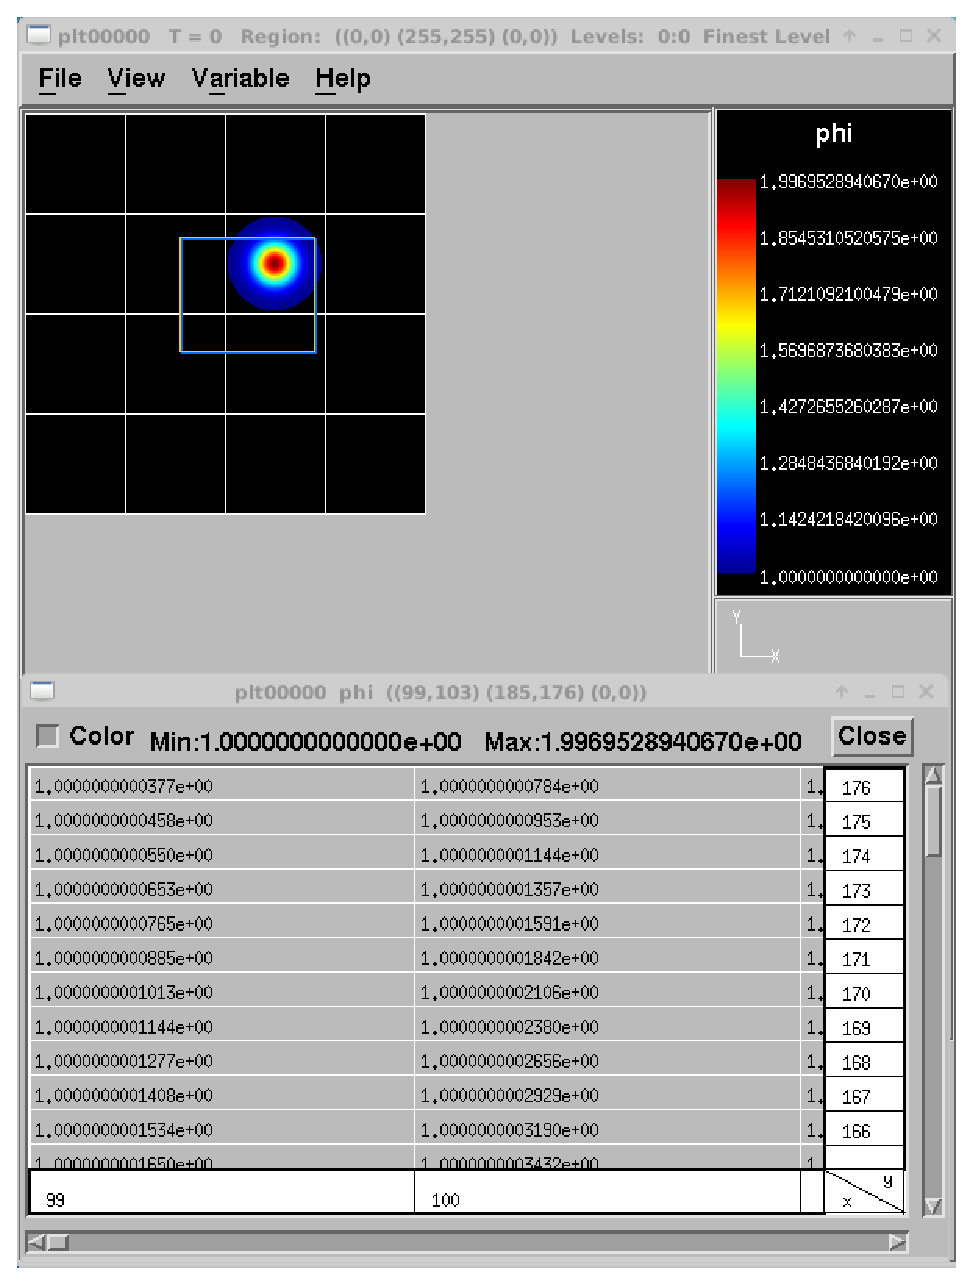
\includegraphics[width=2.5in]{./Visualization/Amrvis_2d}
~~~
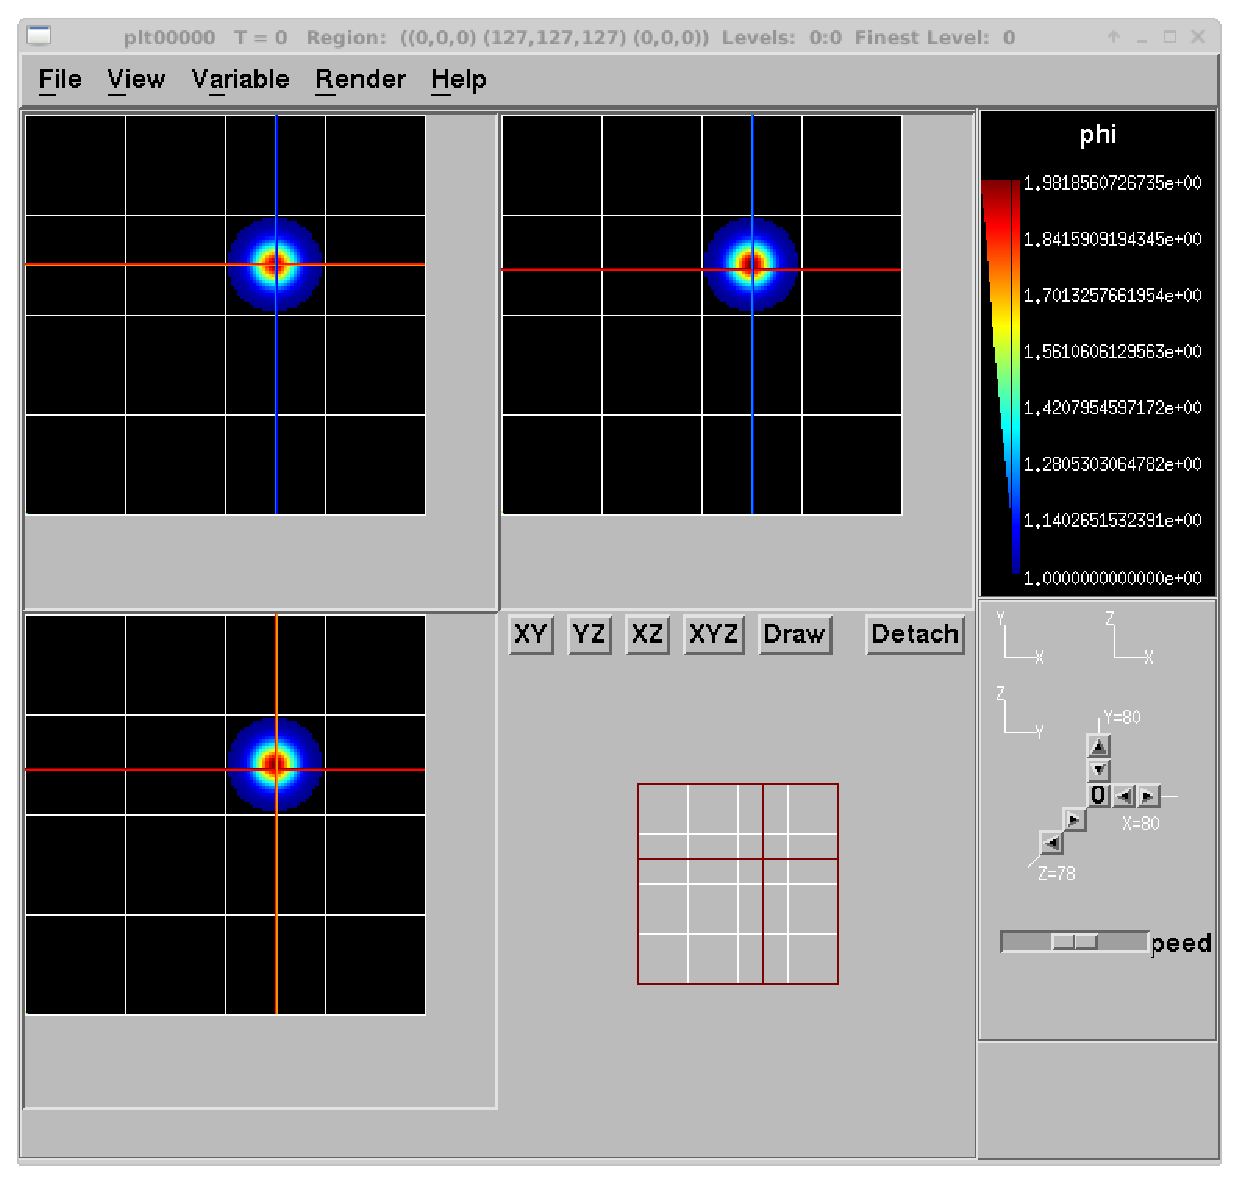
\includegraphics[width=2.5in]{./Visualization/Amrvis_3d}
\caption{2D and 3D images generated with Amrvis}
\label{Fig:Amrvis}
\end{figure}

  We have created a number of routines to convert \amrex\ plotfile data
  other formats (such as MATLAB), but in order to properly interpret 
  the hierarchical AMR data, each tends to have its own idiosyncrasies.
  If you would like to display the data in another format, please contact
  Marc Day ({\tt MSDay@lbl.gov}) and we will point you to whatever we have
  that can help.

\section{\visit}

\amrex\ data can also be visualized by {\tt VisIt}, an open
source visualization and analysis software.  To follow along with this example,
first build and run the first heat equation tutorial code
(see Section \ref{sec:heat equation}).

Next, download and install {\tt VisIt} from \url{https://wci.llnl.gov/simulation/computer-codes/visit}.
To open a single plotfile, run {\tt VisIt}, then select ``File'' $\rightarrow$ ``Open file ...'',
then select the {\tt Header} file associated the the plotfile of interest (e.g., {\tt plt00000/Header}).
Assuming you ran the simulation in 2D, here are instructions for making a simple plot:
\begin{itemize}
\item To view the data, select ``Add'' $\rightarrow$ ``Pseudocolor'' $\rightarrow$ ``phi'', and then select
``Draw''.
\item To view the grid structure (not particularly interesting yet, but when we add AMR it will be), select
`` $\rightarrow$ ``subset'' $\rightarrow$ ``levels''.  Then double-click the text ``Subset - levels'',
enable the ``Wireframe'' option, select ``Apply'', select ``Dismiss'', and then select ``Draw''.
\item To save the image, select ``File'' $\rightarrow$ ``Set save options'', then customize the image format
to your liking, then click ``Save''.
\end{itemize}
Your image should look similar to the left side of Figure \ref{Fig:VisIt}.\\
\begin{figure}[tb]
\centering
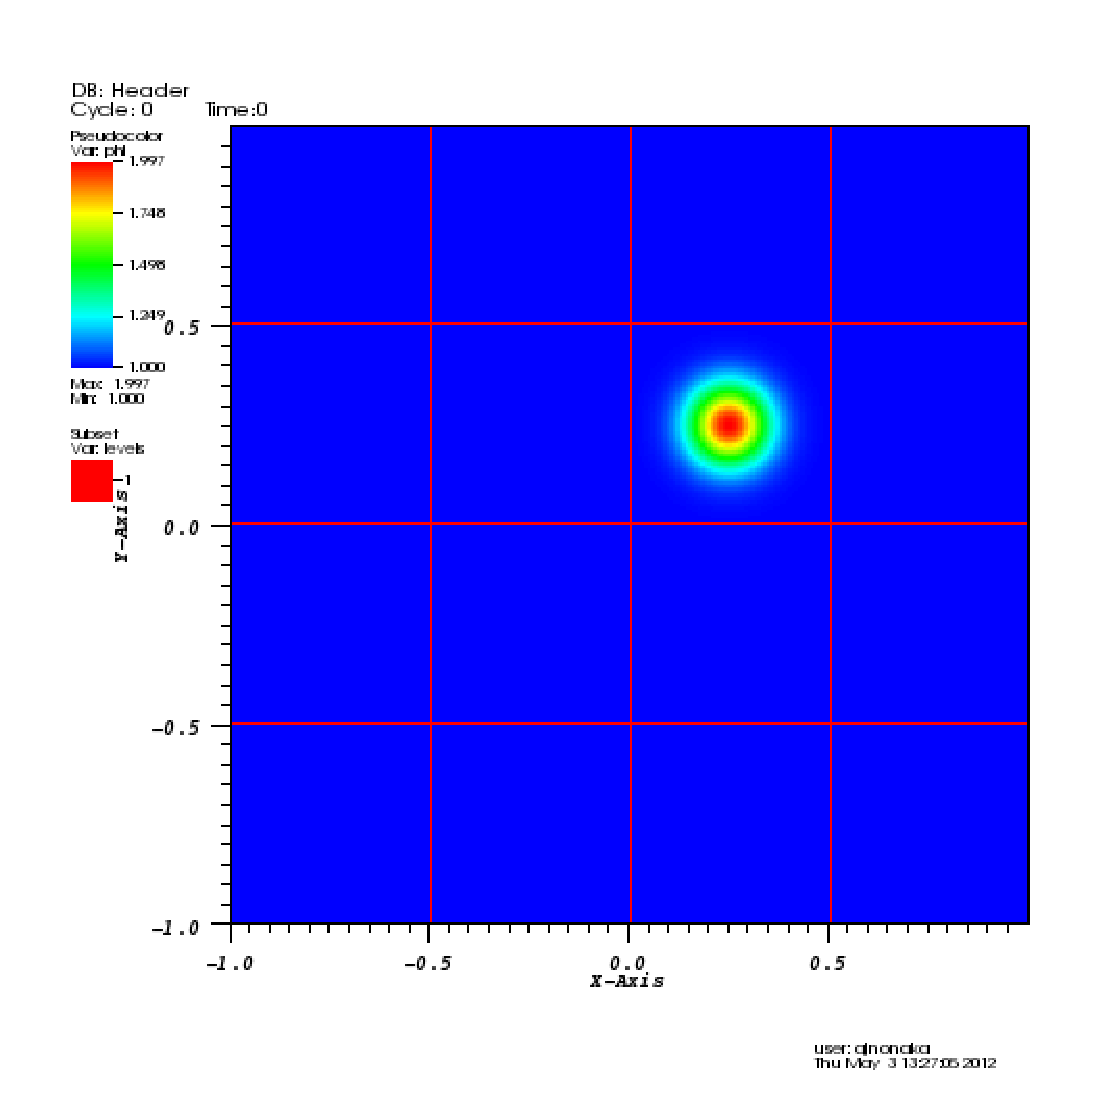
\includegraphics[width=3.1in]{./Visualization/VisIt_2D}
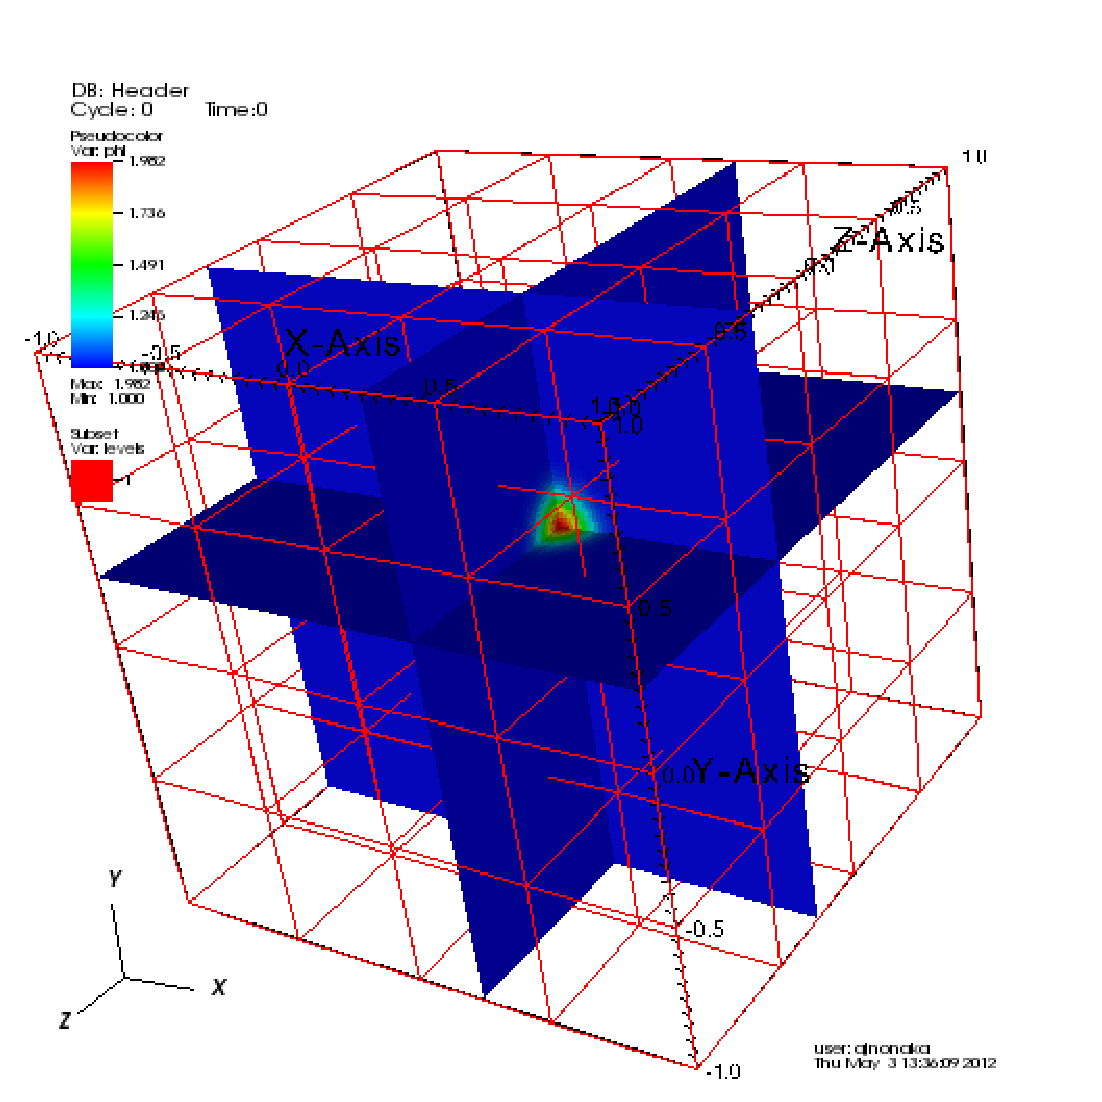
\includegraphics[width=3.1in]{./Visualization/VisIt_3D}
\caption{(Left) 2D image generated with VisIt.  (Right) 3D image generated with VisIt.}
\label{Fig:VisIt}
\end{figure}

In 3D, you must apply the ``Operators'' $\rightarrow$ ``Slicing'' $\rightarrow$ ``ThreeSlice'', with the 
``ThreeSlice operator attribute'' set to x=0.25, y=0.25, and z=0.25.  You can left-click and drag
over the image to rotate the image to generate something similar to right side of Figure \ref{Fig:VisIt}.\\

To make a movie, you must first create a text file named {\tt movie.visit} with a list of the {\tt Header} 
files for the individual frames.  This can most easily be done using the command:
\begin{lstlisting}[backgroundcolor=\color{light-red}]
~/amrex/Tutorials/Basic/HeatEquation_EX1_C> ls -1 plt*/Header | tee movie.visit
plt00000/Header
plt01000/Header
plt02000/Header
plt03000/Header
plt04000/Header
plt05000/Header
plt06000/Header
plt07000/Header
plt08000/Header
plt09000/Header
plt10000/Header
\end{lstlisting}
The next step is to run {\tt VisIt}, select ``File'' $\rightarrow$ ``Open file ...'',
then select {\tt movie.visit}.  Create an image to your liking and press the ``play'' button
on the VCR-like control panel to preview all the frames.  To save the movie, choose
``File'' $\rightarrow$ ``Save movie ...'', and follow the on-screen instructions.

\section{\yt}

{\tt yt}, an open source python package available at
\url{http://yt-project.org/}, can be used for analyzing and
visualizing mesh and particle data generated by \amrex\ codes.  Some
of the \amrex\ developers are also yt project members.

\end{enumerate}
